\chapter{CaseStudy / Evaluation}
\label{ch:CaseStudyEvaluation}

Evaluating our proposed system demonstrates its usefulness in a potential target environment. For the concrete instantiation, the Swift programming language was selected to implement custom subsystems. Required functionality that was already available is integrated using third-party Swift packages. All used packages are published under MIT license. Since it is a prototypical implementation, it supports importing IDLs only for REST-based Web APIs that are described using the OpenAPI specification. Furthermore, its support for generating client libraries is limited to the Swift programming language. 

Section \ref{sec:Implementation} addresses the details of the implementation of \texttt{Pallidor} which is composed of three libraries that are developed and maintained as standalone Swift packages. Each package is described in detail in its respective section, which provides an overview of the package's functionality and public interface. Furthermore, each section details how the package can be integrated into existing applications and shows its current limitations.


For evaluating our proposed system, we perform a migration of two consecutive Web API versions using \texttt{Pallidor}. Therefore, we manually manipulate the OpenAPI specification of the sample \texttt{Pet} \texttt{Store}\footnote{https://petstore3.swagger.io/} Web API so that it reflects all change types we identified. Furthermore, we manually create a machine-readable migration guide for each version of the OpenAPI specification to document all occuring changes. 

The evaluation in Section \ref{sec:Evaluation} is structured according to the degree of automation according to which the respective type of change can be migrated. Changes of the first category, \textsc{Automated Migration}, can be automatically migrated by using \texttt{Pallidor} with our novel machine-readable migration guide. The second category, \textsc{Semi-Automated Migration}, contains changes that can be migrated by \texttt{Pallidor}, but which also require manual intervention by client developers to overcome them. Changes that require new approaches to automating their migration are addressed in the third category, \textsc{Manual Migration}. Each category describes the problems that are caused by the types of change as well as our approach to solving these problems including its benefits and consequences. Each category is concluded by providing our evaluation process and results.

\newpage
\section{Implementation}
\label{sec:Implementation}

For evaluating the proposed system, we created \textit{Pallidor} a prototypical implementation using the Swift programming language. It is composed of multiple subsystems that are developed and maintained as standalone Swift packages. Each package provides the functionality of a subsystem that is defined in Section \ref{ch:SystemDesign}. \texttt{PallidorGenerator} implements the \texttt{IDL Conversion} and \texttt{IDL Importer} subsystems. Migrating a previously generated facade is performed by the \texttt{Pal\-lidor\-Migrator} package that provides the services of the \texttt{Migration Ma\-na\-ger}, \texttt{Migration Guide Importer} and \texttt{SourceCode Importer} subsystems. 

\begin{figure}[!h]
	\centering{
		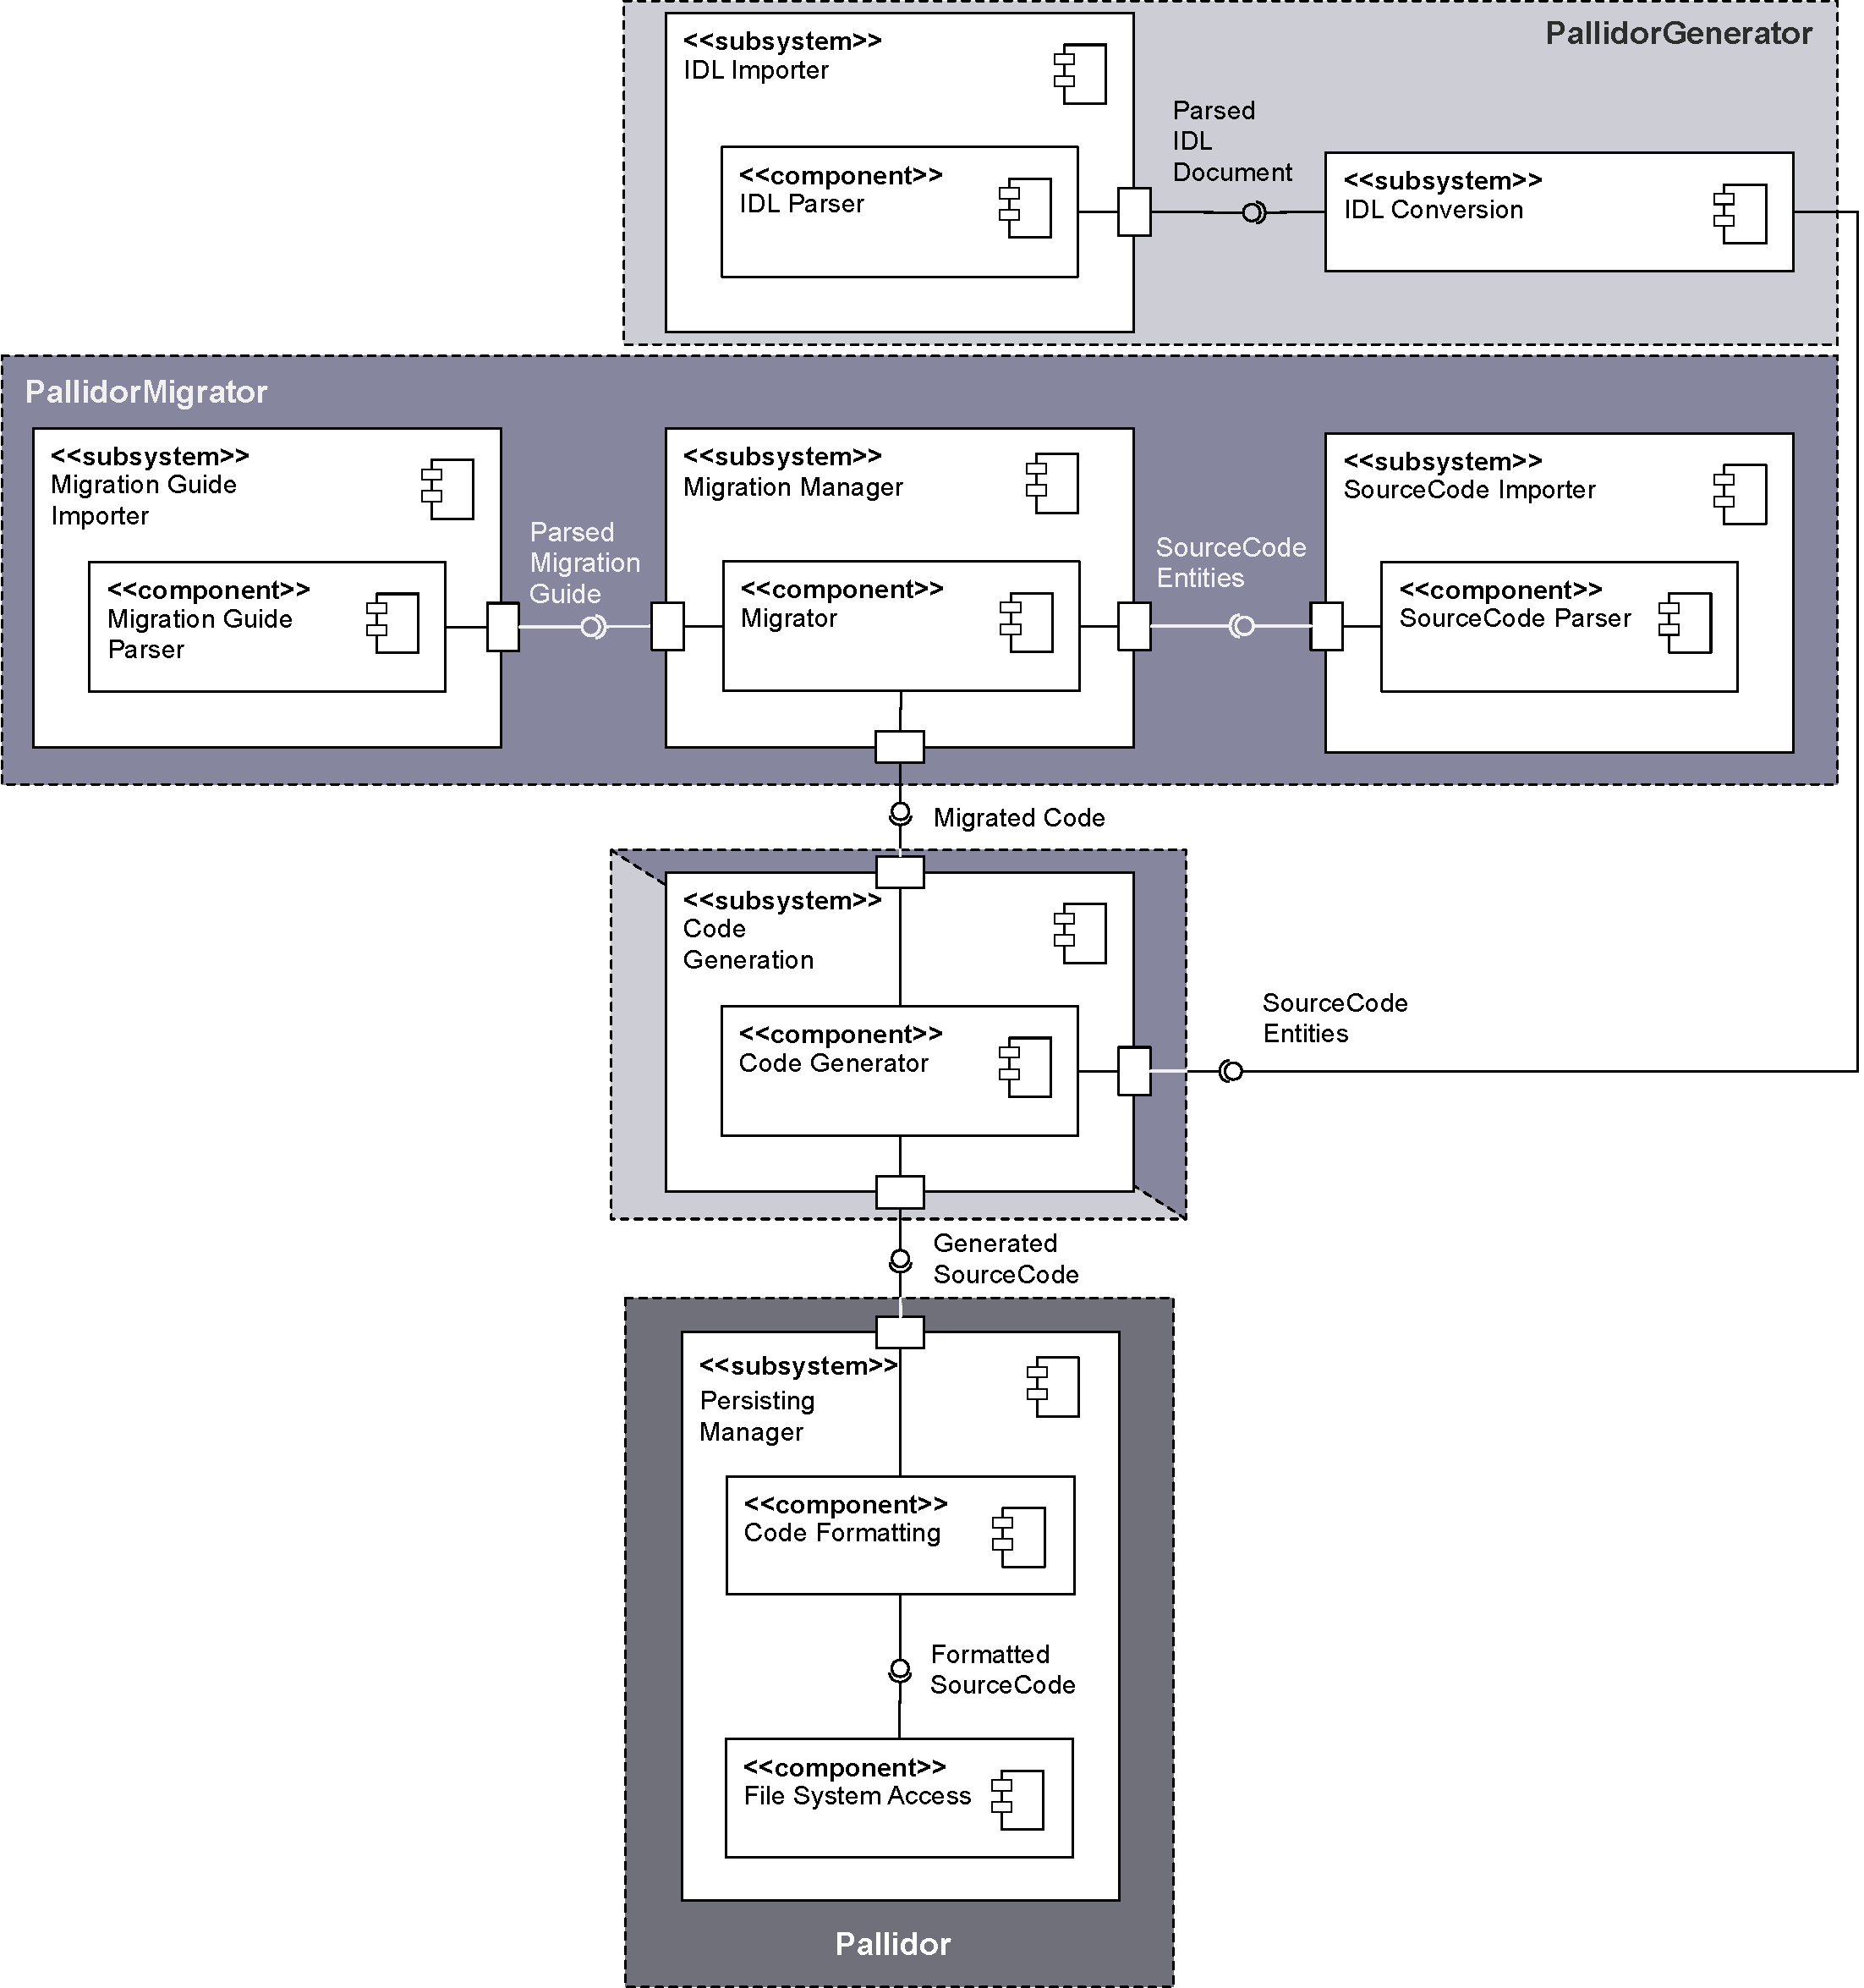
\includegraphics[width=140mm]{images/subsystem_implementation.pdf}
		\caption{Implementation of subsystems with Pallidor Swift packages}
		\label{fig:subsystemImplementation}
	}
\end{figure}
Both packages implement the functionality of the \texttt{Code Generation} subsystem and persist their respective results in files. The \texttt{Code Generation} subsystem is not separately implemented because our prototype only supports the Swift programming language. The \textsc{Pallidor} package combines both subpackages in an executable that provides a command-line user interface. Furthermore, it formats the source code and persists it afterwards. Figure \ref{fig:subsystemImplementation} illustrates which package implements the respective subsystem.  

In addition to our own implementations, third-party open-source components that provide the required functionality are integrated using the Swift Package Manager. Key components and their respective implemented subsystems are listed in Table \ref{tbl:PallidorDep}. Since Pallidor is a prototype, its functionality is limited to generating a persistent Swift package from an OpenAPI specification. It can be integrated in client applications using Swift in version 5.2 or later. Since our generated Swift package uses Apple's \texttt{Combine}\footnote{https://developer.apple.com/documentation/combine} framework, the client application's execution environment must be at least iOS 13 or MacOS 10.15. 

\renewcommand{\arraystretch}{1.4}
\begin{table*}[ht]
	\begin{center}
		\begin{tabular}{|>{\centering\arraybackslash}m{2.7cm}|>{\centering\arraybackslash}m{3cm}|>{\centering\arraybackslash}m{3.2cm}|>{\centering\arraybackslash}m{4cm}|}
			\hline
			\begin{center}
				\textbf{Subsystem/ Component}
			\end{center} &  \begin{center}
				\textbf{Swift Package Name} 
			\end{center}&  \begin{center}
				\textbf{Swift Package Version}
			\end{center} &
		 \begin{center}
			\textbf{Swift Package Author / Publisher}
		\end{center} \\ \hline
			\textit{IDL Importer} & OpenAPIKit & 2.2.0 \newline (Dec. 20th, 2020) &
			Mathew Polzin \\ \hline
			\textit{Source Code Importer} & Sourcery & 1.0.2 \newline (Nov. 30th, 2020) &
			Krzysztof Zabłocki \\ \hline
			\textit{Code Formatter} & swift-format & 0.50300.0 \newline (Sep. 19th, 2020) &
			Apple, Inc. \\ \hline
		\end{tabular}
		\caption{Third-party Swift packages used for subsystems in Pallidor}\label{tbl:PallidorDep}
	\end{center}
\end{table*}

The \texttt{OpenAPIKit} is a library that enables encoding to- and decoding Swift types from OpenAPI documents. It supports importing documents structured in JSON and YAML formats and provides Swift types for most types of the OpenAPI specification in (3.0.2). In its latest version, the \texttt{OpenAPIKit} does not support \texttt{Link Objects} and specification extensions for \texttt{OpenAPI.XML} and \texttt{OpenAPI.Oauth\-Flows}. As opposed to the OpenAPI specification, this library specifies the \texttt{re\-qui\-red} property of schema elements on the element instead of the parent object. OpenAPI documents must be provided as \texttt{Data} or \texttt{String} types, as the \texttt{OpenAPIKit} does not support reading files. Furthermore, all reference elements (\texttt{\$ref}) must be internal references and target the same file in order to be resolved.

\texttt{Sourcery} is a code generator for Swift, built on top of Apple's \texttt{SourceKit}. It extends its functionality and types to facilitate generating Swift code based on Stencil templates. Although \texttt{Sourcery} is designed as a command-line tool to be integrated in a custom build phase, it provides a framework that can be incorporated using the Swift Package Manager. In addition to generating Swift code, it provides support for parsing Swift strings in corresponding source code entities. 

Formatting the generated Swift code is performed by \texttt{swift-format}. It can be used as a command-line tool or integrated into applications using the Swift Package Manager. It provides an API to format Swift code according to a style configuration. If no set of styling rules is specified, a default style is used. The package is compatible with Swift 5.1 and higher and requires selecting the appropriate branch that corresponds to the version of Swift used in the integrating application.

\subsection{Pallidor Generator}\label{subsec:PallidorGenerator}

The \texttt{PallidorGenerator} Swift package is concerned with retrieving and parsing of OpenAPI specifications to generate the library layer of the Swift package for the client application. Therefore, OpenAPI specifications must be parsed and converted to source code entities. After that, they are transformed into source code strings in the Swift programming language and are persisted in files. The package integrates the \texttt{OpenAPIKit} which decodes an OpenAPI specification in its \texttt{Open\-API.Document} type. This type is composed of elements that represent the attributes of an OpenAPI specification. Furthermore, it provides a locally dereferenced representation that facilitates the traversal of its structure by replacing all \texttt{\$ref} elements with their referenced entities. The \texttt{OpenAPI.Document} needs to be converted to source code entities before Swift code can be generated. This conversion is performed during the traversal of the document by using various \texttt{Resolver} objects. Depending on the OpenAPI specification element that needs to be converted, a corresponding \texttt{Resolver} initializes a source code entity model using the information of the OpenAPI element. Resolving an endpoint struct from the \texttt{Resolved\-Route} type of the \texttt{OpenAPIKit} is shown in Listing \ref{lst:Resolving}.

\begin{lstlisting}[language=Swift, caption={Resolving an operation}, captionpos=b, label={lst:Resolving}]
	/// Resolves an endpoint struct
	/// - Parameters:
	///   - path: path in OpenAPI document
	///   - route: Resolved route from OpenAPI document
	/// - Returns: resolved EndpointModel
	static func resolve(path: OpenAPI.Path, route: ResolvedRoute) -> EndpointModel {
		let endpoint = EndpointModel(
				name: path.components[0].upperFirst(), 
				operations: [], 
				detail: route.summary)
		endpoint.operations = route.endpoints.map( 
				{ OperationModel.resolve(endpoint: $0) })
		return endpoint
	}

\end{lstlisting}

All source code entity models of the \texttt{PallidorGenerator} package are extended with the \texttt{Custom\-String\-Convertible} protocol that adds the \texttt{description} computed property. It is used to specify string templates for generating the Swift code of the library layer. They are dynamically composed of all string templates of nested models such as methods, parameters or properties. Furthermore, static templates for meta files such as the \texttt{Package.swift} file are provided as Markdown (\texttt{.md}) files. Although minor adjustments are made, for example specifying the name of the Swift package, their functionality remains the same between different Web APIs.

\begin{lstlisting}[language=Swift, caption={Source code string template for an endpoint}, captionpos=b, label={lst:EndpointTempl}]
	/// Extension of the Endpoint Model
	/// Used for generating client library code in Swift
	extension EndpointModel : CustomStringConvertible {
		var description: String {
			"""
			import Foundation
			import Combine
			
			struct _\(name.upperFirst())API {
				static let decoder ...
				\(operations
				.sorted(by: {$0.operationId < $1.operationId})
				.map({$0.description})
				.joined())
			}
			"""
		}
	}

\end{lstlisting}

The public interface of the \texttt{PallidorGenerator} Swift package is provided by the file of the same name. Its initialization requires specifying the URL of the OpenAPI specification to be decoded. Depending on its format, a \texttt{JSON\-Decoder} or \texttt{YAML\-Decoder} is created that is used to decode the OpenAPI specification. Initializating the \texttt{Pal\-li\-dor\-Gen\-er\-ator} fails, if the OpenAPI document cannot be decoded or resolved due to an invalid URL or malformed structure. Generating the Swift code of the library layer and persisting it in files is performed by invoking its \texttt{generate} method. It receives a \texttt{path} parameter and the name of the client library as specified by the user. After generating all files, a list of their URLs is returned to the method's caller. The method throws an error if writing the files in the target directory fails. Several OpenAPI specifications of various Web APIs are used for testing the \texttt{PallidorGenerator} Swift package. They are specified in Markdown files and are located in the \texttt{Resources} subfolder of the test folder. The generated files are validated against predefined results specified in Markdown files that are located in the \texttt{Results} subfolder. 

Integrating the \texttt{PallidorGenerator} package in a Swift project, the URL of its GitHub repository must be added to the dependencies in the \texttt{Package.swift} file. Furthermore, the \texttt{develop} branch must be selected for using its latest version.
\newpage
\begin{lstlisting}[language=Swift, caption={Integrating PallidorGenerator in SPM}, captionpos=b, label={lst:IntegrationGenerator}]
	.package(
			url: "https://github.com/Apodini/PallidorGenerator.git", 
			.branch("develop")
	)
\end{lstlisting}


With regard to the implementation of the \texttt{PallidorGenerator} Swift package, some restrictions must be observed. Instead of defining inline objects in nested elements of an OpenAPI specification, schema components must be used to specify custom data types. They must be referenced at their designated target element. This limitation is based on the problem that nested elements do not provide an identification, which is required for building the library layer. The Open\-API specification supports defining primitive data types as schema components using a custom name. These type aliases are resolved and their underlying primitive types are used in the generated client library. Furthermore, all endpoint methods in an Open\-API specification must specify the \texttt{operationId} property. Analogous to schema components, this identifier is used by \textsc{Pallidor} to recognize changes and to generate the client library. Although it is not enforced by the OpenAPI specification, all operations must specify at least one response that is returned after the request was processed successfully. Otherwise the return value type of an operation cannot be inferred from the Open\-API document. Unlike successful responses, error responses can be of various types.
\subsection{Pallidor Migrator}\label{subsec:PallidorMigrator}

The \texttt{PallidorMigrator} package integrates the functionality of the \texttt{Migration} \texttt{Ma\-nager}, \texttt{Migration Guide Importer} and \texttt{SourceCode Importer} subsystems. It uses the information stated in the parsed migration guide to adapt the source code entities of a previously generated facade layer. Therefore, a set of migrations is initialized that performs the necessary migratory steps on the changed target properties of the source code entity. After migrating all changes, the source code entities are converted into Swift code that gets persisted in files. The machine-readable migration guide is parsed by the builtin \texttt{JSONDecoder} of Swift's \texttt{Foundation} framework. The \texttt{PallidorMigrator} package provides a model for mapping the migration guide to its decoded representation. Depending on the type of change that is stated in the migration guide, the \texttt{MigrationSet} initializes a corresponding \texttt{Migration} object. Each \texttt{Migration} is checked for plausiblity on its initialization. Thereby, invalid or inconsistent changes are detected and its \texttt{solvable} property is set to false. An unsolvable \texttt{Migration} results in an error message that is propagated to the user. Every \texttt{Migration} targets one source code entity of a previously generated facade. The \texttt{Sourcery} framework is used for importing its source code. It provides source code entities for all syntactical elements of Swift code such as classes, structs and methods. These entities cannot be extended within the \texttt{PallidorMigrator} package, because they are declared as \texttt{final}.

\begin{lstlisting}[language=Swift, caption={Extending a wrapped Sourcery struct}, captionpos=b, label={lst:WrappedStruct}]
	/// Wraps struct types of Sourcery
	class WrappedStruct: Modifiable {
		...
		convenience init(from: SourceryRuntime.Struct) {
			self.init(
				localName: from.localName.removePrefix, 
				variables: from.variables
					.map({ WrappedVariable(from: $0) }), 
				methods: from.methods
					.map({ WrappedMethod(from: $0) }))
		}
	}
\end{lstlisting}

In order to adapt them to changes, wrapper classes are used to extend their functionality with the \texttt{Modifiable} protocol. This protocol introduces a \texttt{modify} method that receives a \texttt{Change} object as a parameter. A modifiable endpoint struct that wraps the \texttt{SourceryRuntime.\-Struct} type of the \texttt{Sourcery} framework is shown in Listing \ref{lst:WrappedStruct}. Depending on the type of change that the \texttt{modify} method receives, the corresponding handling routine is performed. 

\begin{lstlisting}[language=Swift, caption={Modification of a changed method entity}, captionpos=b, label={lst:MethodModify}]
	/// Wrapped method of SourceryMethod
	class WrappedMethod: Modifiable {
		...
		func modify(change: Change) {
			self.modified = true
			switch change.changeType {
				case .add:
					handleAddChange(change: change as! AddChange)
					break
				case .rename:
					handleRenameChange(change: change as! RenameChange)
					break
				case .replace:
					handleReplaceChange(change: change as! ReplaceChange)
					break
				case .delete:
					handleDeleteChange(change: change as! DeleteChange)
					break
			}
		}
	}
\end{lstlisting}

Their implementations vary depending on the type of source code entity that is modified. They adapt an entity's associated properties according to the details of the migration. In Listing \ref{lst:MethodModify}, the implementation of the \texttt{modify} method highlights the various handling routines that are used to migrate the properties of a \texttt{WrappedMethod}. Similar to the source code entities of the \texttt{PallidorGenerator} package, the wrapped source code entities provide templates that are used to convert them into Swift code. These source code strings are persisted in files.

The public interface of the \texttt{PallidorMigrator} Swift package is provided by the file of the same name. Its initialization requires specifying the URL of the migration guide and the URL of the directory in which the previously generated client library is located. If the migration guide cannot be retrieved or decoded, an error message is thrown and forwarded to the user. Furthermore, on initialization of the \texttt{PallidorMigrator} struct a set of migrations is created. If their plausibility check fails, an error message is shown to the user. Migrating the changes as stated in the migration guide and persisting the adapted facade layer in files are started by invoking the \texttt{buildFacade} method. After generating all files, it returns a list of their URLs. An error is thrown if writing the files of the adapted facade layer fails. The \texttt{PallidorMigrator} Swift package is extensively tested to discover erroneousness migrations. Therefore, migration guides are created that contain various types of changes with their respective targets. The unit tests migrate prepared source code entities according to these migration guides and compare the outcome to predefined results. Various integration tests are performed that combine different changes on a single target to ensure that they do not affect each other. The input documents of previously generated facade layer code and their predefined adapted results are specified in Markdown files located in the \texttt{Resources} subfolder of the test folder. 

Integrating the \texttt{PallidorMigrator} package in a Swift project, the URL of its GitHub repository must be added to the dependencies in the \texttt{Package.swift} file. Furthermore, the \texttt{develop} branch must be selected for using its latest version.

\begin{lstlisting}[language=Swift, caption={Integrating PallidorMigrator in SPM}, captionpos=b, label={lst:IntegrationMigrator}]
	.package(
		url: "https://github.com/Apodini/PallidorMigrator.git", 
		.branch("develop")
	)
\end{lstlisting}

The implementation of the \texttt{PallidorMigrator} Swift package deviates from the design of our proposed system. In addition to the original design, the generated library layer must also be imported. No migration guide or previously generated facade can be used during the initial integration of \textsc{Pallidor} as the current version of the Web API is persisted. Therefore, the facade layer is generated based on the public interface of the library layer. Furthermore, no migration strategy can be selected so that all changes of a WebAPI are migrated. A limitation of \texttt{Sourcery} concerns the automatic documentation of the public facade layer of the client library because it does not support parsing comment annotations. Therefore, the documentation for the client library is located at the library layer and must be consulted manually. Additionally, some types of migration must be performed by combining multiple migratory steps. Replacing an endpoint is achieved by replacing all of its methods and then renaming it. Renaming and replacing enum cases and inherited schemas is accomplished by adding their replacements before removing them. Return values of endpoint methods can only be replaced because they do not specify a name that could be renamed. Furthermore, all operations must provide a return value type, which means that deleting them or adding them later is not applicable.
\subsection{Pallidor}\label{subsec:Pallidor}
The \textsc{Pallidor} package contains the command-line user interface and the \texttt{Code\- Formatting} component. Furthermore, it stores all configuration settings of the user. By invoking \textsc{Pallidor} via its commandline interface and providing all required configuration parameters, the client library is generated. The \texttt{swift\-argument-parser}\footnote{https://github.com/apple/swift-argument-parser} package is used to supply detailed error and help messages and it facilitates type-safe argument parsing. The URLs of the OpenAPI specification and migration guide are used to initialize the \texttt{Pallidor\-Generator} and \texttt{Pallidor\-Migrator} Swift packages. Additionally, the name and location of the client library are used by the packages to both, import previously generated source code and persist their results after execution. After both packages successfully completed their tasks, the \texttt{swift-format} package is used to format the code according to the ruleset that the user provided. The formatted source code strings overwrite the previously generated Swift files.

Several parameters are used to configure \textsc{Pallidor}. While the URLs of the migration guide, OpenAPI specification and location of the package as well as its name are mandatory parameters, specifying a ruleset for formatting the source code strings is optional. \textsc{Pallidor} is limited to emitting the client library as a Swift package, hence selecting a programming language currently defaults to Swift. A migration strategy can be set to exclude certain types of migration. This configuration parameter defaults to the implemented strategy of migrating all types. The \texttt{help} argument is provided by the \texttt{swift-argument-parser} and lists all available parameters of \textsc{Pallidor}. It also supports the user with helpful error messages that highlight the correct usage.

\begin{lstlisting}[language=Tex, caption={Command-line arguments of Pallidor to support user}, captionpos=b, label={lst:arguments}]
	Error: Missing expected argument 
				'--target-directory <target-directory>'
	
	USAGE: pallidor 
	--openapi-specification-url <openapi-specification-url> 
	--migration-guide-url <migration-guide-url>
	--target-directory <target-directory> 
	--package-name <package-name> 
	[--language <language>] 
	[--strategy <strategy>]
	[--custom-formatting-rule-path <custom-formatting-rule-path>]
	
	OPTIONS:
	-c, --custom-formatting-rule-path <custom-formatting-rule-path>
	If you want to use your own code formatting rules, specify path here 
	-o, --openapi-specification-url <openapi-specification-url>
	URL of OpenAPI specification of the package to be generated 
	-m, --migration-guide-url <migration-guide-url>
	URL of migration guide of the package to be generated 
	-t, --target-directory <target-directory>
	Output path of the package generated 
	-p, --package-name <package-name>
	Name of the package generated 
	-l, --language <language>
	Programming language that the client library should be generated in (default: Swift)
	-s, --strategy <strategy>
	Migration strategy that excludes certain types of change from being migrated (default: all)
	-h, --help
	Show help information.

\end{lstlisting}

\textsc{Pallidor} is designed as a command-line tool that can be integrated into an existing CI/CD system. Therefore, it needs to be compiled and the binaries must be deployed. The configuration parameters can be predefined in a script file that is integrated in the build phase of the CI pipeline. The script is automatically executed as a step phase and performs the migration to generate the Swift package that is integrated in the client application. The CI/CD system must be configured to publish the generated Swift package in a separate respository that is referenced from the \texttt{Package.swift} file of the client application. After that it automatically creates a new release of the client application.



\newpage
\section{Evaluation}
\label{sec:Evaluation}
For evaluating our proposed system, we use IDL documents of two consecutive Web API versions and a corresponding migration guide. The IDL documents must be manually manipulated as they only describe the latest version of a Web API. Since a machine-readable migration manual is neither publicly available nor can it be generated automatically, it must be created manually in order to document all occuring changes. Most changes cannot be viewed in isolation, as changes to higher-level elements affect changed sub-elements. For a thorough assessment of our proposed system's capability to migrate the various changes and their permutations, we decided to perform the evaluation by manually incorporating them in the sample \texttt{Pet} \texttt{Store}\footnote{https://petstore3.swagger.io/} Web API. Therefore, its OpenAPI specification is modified to reflect the change patterns that were discovered by Li et. al \cite{li_how_2013}. Additionally, migration guides are created for each type of migratable change and permutation that provide instructions on how to overcome the breaking change. 

The documentation of our results is based on the structure of the 
\textit{Deductive Mini-Pattern} template, that focuses the outcomes of the described solution including the respective benefits and consequences \cite{brown_refactoring_1998}. The different types of changes are separated into the categories \textsc{Automated Migration}, \textsc{Semi-Auto\-mated Migration}, and \textsc{Manual Migration} depending on their degree of automation. Furthermore, they share commonalities in the problems they cause for client applications and their developers. These problems are presented in detail for each category to clarify the necessity of their solution. In the description of the respective solution, we explain the different approaches that support client developers in migrating their application. Each solution offers individual benefits, but also has other consequences. By describing the benefits of a solution, we focus on the positive effects of our system on the reduction of the effort required for the manual migration for client developers. The consequences described serve as support for users of our system, since observing them helps preventing undesired side effects in the client application. Finally, we describe the testing procedure and the required documents used in this process.

\subsection{Automated Migration}\label{subsec:EvalAutomated}
Breaking changes that belong to this category result in compile-time errors because they affect syntactical elements of the client library. They are always reflected in a Web APIs IDL document and currently require manual refactoring activities by client developers. In the course of this, client developers must consult all related documents in order to integrate the changes into their application accordingly. By using \texttt{Pallidor} with our novel machine-readable migration guide, this process can be fully automated.
\newpage
\begin{description}
	\item[Category:] \textsc{Automated Migration} \newline Automating the migratory steps is based on two approaches. The first approach is to automatically adapt the client library to the changes in the migration guide. The second approach is the implementation of the separation of concerns principle through the encapsulated design of the client library.
	\item[Problem:] All of the changes in this category require refactoring the client application. Depending on whether the client application uses a wrapper library or accesses the Web API directly via HTTP request, these changes cause an error at compile time or runtime. Breaking changes of this category are listed below:
	\begin{itemize}
		\item \textit{Renaming} changes of models, attributes, parameters, methods or endpoints alter the identifier of the syntax elements without modifying other related properties or their behavior. They require client developers to adapt their application to use the new identifiers. Although modern \acp{IDE} provide support for automatically renaming all occurrences of a syntax element, a client developer must manually start this process. Renaming migration tests are listed in Table \ref{tab:RenameMigrationTests}.
		\item \textit{Replacing} changes of models, attributes, parameter and methods are reflected in the IDL document by the removal of the element. In contrast to a \textit{Removing} change, a replacement for the removed element is provided, which can be specified in other related documents. Client developers must manually inspect these documents in order to find the replacement that can be used in their application. This examination is cumbersome for Web API consumers because according to Brito et. al, providers do not use a single artifact for documenting changes \cite{brito_you_2020}. Automating the migration of a \textit{Replace} change requires Web API providers to specify the replaced element and its replacement in the machine-readable migration guide. Furthermore, they must provide algorithms for converting and reverting types of a replaced model, attribute or a methods parameters and return values using the Javascript programming language. All tests that concern replacements of all target types are listed in Table \ref{tab:ReplaceMigrationTests}.
		\item \textit{Permutations} of changes are not described by Li et. al \cite{li_how_2013} but they introduce multiple side effects that need to be considered. For example when replacing a parameter of a method is followed by a \textit{Renaming} change of its signature, the latter must be migrated before replacing the parameter. \textit{Permutations} can occur for all types of changes with the exception of \textit{Removing} changes, because removing the parent element has the same effect on all child elements. \textit{Permutations} significantly increase the effort involved in manually migrating a client application. \texttt{Pallidor} requires Web API providers to state changes that affect others in a specific order that is shown in Table \ref{tab:ChangeOrder}.
		\item \textit{Combining and splitting methods} extends the problem of a single replacement for a removed method. By combining the functionality of multiple methods in a single method, the parameters of the replaced methods must be combined before invoking the replacement. Its return value must be split to match the return values of the replaced methods. By splitting a single method into multiple methods, its parameters are split and the return values of all replacements must be combined before returning the result. This type of change is currently not supported by \texttt{Pallidor} but it can be extended to add this feature.
		\item \textit{Combining and splitting parameters} are an extension of single replacements for parameters. Combining multiple independent parameters of a primitive type to a complex type can be migrated by synthesizing the new type from the previous types. This may be complemented by a change in the underlying HTTP method that allows transmitting a content body. For splitting a complex type into multiple primitive types, it must be decomposed before invoking the method.
		\item \textit{Changing default value of parameters} does not prevent the client application from compiling as default values are only applicable to optional parameters. However, when client developers use a parameters default value, changing it can result in unexpected behavior. For example, if a parameter specifies the number of elements returned from the Web API, changing the default number affects the number of displayed elements in the UI of a client application.
		\item \textit{Adding required parameters} or requiring a previously optional parameter change the conditions of invoking a method and must be migrated. Therefore, Web API providers must specify a default value that can be used to call the method in case no value is passed by the client developer.
		\item \textit{Adding} models, attributes, optional parameters, methods or endpoints does not break client applications as they introduce new functionality without modifying existing services. However, these additions should be made available to client developers to extend their applications. The test cases of both adding change types are listed in Table \ref{tab:AddMigrationTests}.
		\item \textit{Changing the underlying HTTP method} results in an error message returned by the server. Depending on the architecture of an application, this change can affect multiple files that must be modified by client developers. By encapsulating lower-level HTTP calls, this type of change only affects one file. 
		\item \textit{Changing the servers URL or ports} result in an error message of the client application. As with changing the underlying HTTP method, the client applications architecture has a decisive influence on the effects of this change. Impacts on security systems such as firewalls are ignored in our evaluation.
	\end{itemize}
\newpage
\item[Solution:] For migrating the changes of the underlying HTTP method and the servers URL or ports, we designed the architecture of the client library to automatically incorporate these changes. Therefore, the \texttt{NetworkManager} struct in the library layer encapsulates lower-level HTTP calls and contains a list of server URLs that is extracted from the OpenAPI specification. By default, the first server in the list is selected to state requests to the Web API. The library layer specifies the HTTP method that is used to query the Web APIs endpoints. The facade layer only invokes the higher-level methods of the library layer, hence the client application remains its functionality regardless of these changes in the library layer. New services are automatically integrated in the client library and do not require an entry in the migration guide.   All other changes cannot be incorporated by design and must be migrated. Therefore, \texttt{Pallidor} uses the information of the machine-readable migration guide to instantiate a \texttt{MigrationSet} that contains all \texttt{Migrations} that need to be performed. Migrating a change is executed by adapting the target syntax elements of the facade layer to incorporate the changes of the library layer.
\item[Benefits:] By automating the refactoring process, the effort for client developers is significantly reduced. By concentrating all evolution-related information in a machine-readable migration guide the necessity of manually examining related documents of the Web API is eliminated. Client developers are able to integrate \texttt{Pallidor} into their CI workflow which ensures that their application always incorporates the latest changes of a Web API dependency. 
\item[Consequences:] Using our solution enables client developers to operate their application on an outdated syntax of the Web API. Some changes require fallback or default values in order to be migratable and they may not contain the specific values required by the client developer. Migrations of \textit{Replacing} changes need to execute foreign code which reduces the applications performance and raises security concerns. By migrating the combination or splitting of methods instead of using the implementation of the Web API, client applications cannot benefit from potential increases in performance and efficiency.
\item[Tested By:] All change types of this category are tested by unit tests or executable script files. Each change type is tested on a target in isolation and also in combination with other change types if this applies for the target type. In the remainder of this section, the test cases for all change types are listed in their respective table except for the \textit{Permutation} change types which can be found in the Appendix \ref{tab:PermutationAPITests} and \ref{tab:PermutationModelTests}. All tables in this section list the performed tests on each target type. The tests are either given as unit tests or they refer to a script that can be locally executed from the root directory of the \texttt{Pallidor} Swift package. They require to specify the target directory of the generated Swift files using the \texttt{-t} parameter. Each script generates separate Swift packages for the unchanged and updated version of the Web API to facilitate the comparison of the changed elements. Script files are highlighted in \textit{italic} while unit tests are prefixed with the \texttt{test} keyword.
\end{description}

New elements of a Web API are incorporated either by the design of the generated Swift package or by automatically adding them during the migration process. Adding new attributes or required parameters must be migrated as they break the client application. New functionality such as adding models, methods and endpoints is automatically integrated in the library and facade layer of the Swift package. Methods must specify a return value as described in Section \ref{subsec:PallidorGenerator}, hence return values cannot be added after publishing the Web API.

\begin{table}[!ht]
	\begin{center}
	\begin{tabular}{@{}lp{0.18\textwidth}p{0.17\textwidth}p{0.4\textwidth}@{}}
		\toprule
		\textbf{Target} & \textbf{Test} & \textbf{Identifier} & \textbf{Description} \\ \midrule
		Model           &   \textit{addModel.sh} &    \multicolumn{1}{c}{-}      &   The \texttt{ApiResponse} model gets automatically integrated in the Swift package. No migration guide is required as this is a non-breaking change. However, any replacement changes that are referencing the new type must be stated in a migration guide.  \\
		Attribute       &   test\-Added\-Property   &    \texttt{city}      &      A new attribute is added to the \texttt{Address} model. It specifies a default value to prevent en-/decoding errors       \\
		Endpoint        &          \textit{addEndpoint.sh} &    \multicolumn{1}{c}{-}      &            The \texttt{Store} endpoint gets automatically integrated in the Swift package. No migration guide is required as this is a non-breaking change.                               \\
		Method        &         \textit{addMethod.sh}  &    \multicolumn{1}{c}{-}      &            New methods are automatically integrated in the respective endpoint of the facade layer.                      \\
		Parameter       &               test\-Added\-Parameter                    &    \texttt{status}                        &       A new required parameter \texttt{status} is added to \texttt{updatePet}.             \\
		Return Value    &            \multicolumn{1}{c}{-}  &    \multicolumn{1}{c}{-}                   &      Due to our predefined constraints, return values must be available for each method. Adding a new return value is therefore not valid.         \\ \bottomrule
	\end{tabular}
	\caption{Adding migrations for all target types}
	\label{tab:AddMigrationTests}
		\end{center}
\end{table}

Depending on whether a wrapper library is used to access the Web API or it is queried directly, renaming elements either leads to compiler errors or error messages returned from the Web API. Refactoring is performed by modifying the internals of the facade layer to use the new identifiers in the library layer. However, the public interface of the facade layer is not changed. Return values have no identifier, hence renaming them is infeasible. Changes in models affect other elements of the Web API as they are used as types by parameters, return values or attributes. In order to rename them, the Web API provider must replace the types of the affected elements accordingly.

\begin{table}[!ht]
	\begin{center}
		\begin{tabular}{@{}lp{0.18\textwidth}lp{0.4\textwidth}@{}}
			\toprule
		\textbf{Target} & \textbf{Test} & \textbf{Identifier} & \textbf{Description} \\ \midrule
			Model           &   test\-Renamed\-Model  &    \texttt{Address}     &   Renamed the \texttt{Address} model to \texttt{NewAddress}. Changing the identifier of a model requires to replace the types of all referencing elements. Therefore, also a replace change of the \texttt{address} attribute of the \texttt{Customer} model is migrated.    \\
			Attribute       &   test\-Renamed\-Property   &  \texttt{tags} \texttt{\&} \texttt{name}      &      The attributes of  \texttt{Pet} and \texttt{Category} are renamed to \texttt{tagsi} and \texttt{namenew}.    \\
			Endpoint        &     test\-Endpoint\-Renamed  &    \texttt{/pet}     &   The route of the Pet endpoint is changed to \texttt{/pets}. This results in a renaming change from \texttt{PetAPI} to \texttt{PetsAPI}.     \\
			Method        &     test\-Renamed\-Method     &    \texttt{addPet}    &           The method is renamed to \texttt{addMyPet}.                            \\
			Parameter       &               test\-Renamed\-Parameter                    &    \texttt{status}       &       The parameter of \texttt{findPetsByStatus}  is renamed to \texttt{petStatus}        \\
			Return Value    &            \multicolumn{1}{c}{-}  &    \multicolumn{1}{c}{-}                   &      Return values do not have an identifier and hence cannot be renamed.         \\ \bottomrule
		\end{tabular}
		\caption{Rename migrations for all target types}
		\label{tab:RenameMigrationTests}
	\end{center}
\end{table}
\vspace{-0.5cm}
In addition to renaming their identifiers, replacing Web API element also changes their types. In order to maintain a stable public interface of the facade layer, the previously used types must be converted to their replacement types and the replacement types must be reverted to their original types. Therefore, Web API providers must specify the respective algorithm in the migration guide using the Javascript programming language. When a method is replaced, the conversion algorithm is used to convert the parameters of the original method to an object of the parameters of its replacement. The reverting algorithm is used to convert the replacements return type back to the original return type. Replacing an endpoint cannot be specified as a dedicated change type in our migration guide. However, to replace an endpoint, its identifier can be renamed after all of its methods were replaced.

		\begin{longtable}{@{}lp{0.18\textwidth}lp{0.4\textwidth}@{}}
			\toprule
		\textbf{Target} & \textbf{Test} & \textbf{Identifier} & \textbf{Description} \\ \midrule \endfirsthead
		\toprule
		\textbf{Target} & \textbf{Test} & \textbf{Identifier} & \textbf{Description} \\ \midrule \endhead
			Model           &   test\-Replaced\-Model  &    \texttt{Order}     &   Replaced the \texttt{Order} model by \texttt{NewOrder}.  In contrast to renaming a model, algorithms for converting and reverting must be specified. Replacing a model requires to use the \texttt{Signature} target value of changes. \\
			Attribute       &   test\-Replaced\-Property   &  \texttt{address}   &      The attribute was renamed to \texttt{addresses} and also its type is changed to \texttt{[NewAddress]}.    \\
			Endpoint        &  \multicolumn{1}{c}{-}     &    \multicolumn{1}{c}{-}    &   Endpoints can not be directly replaced using our migration guide. Replacing an endpoint is performed by replacing all of its methods before renaming the endpoint.     \\
			Method &    test\-Replaced\-Method   &    \texttt{updatePet} &     The method is replaced by \texttt{updateMyPet} in the \texttt{User} endpoint. Replacing a method requires to use the \texttt{Signature} target value of changes.                       \\
			 &   test\-Replaced\-Method\-InSame\-Endpoint   &    \texttt{updatePet} &     The method is replaced by \texttt{updatePetWithForm} in the \texttt{Pet} endpoint. Replacing a method requires to use the \texttt{Signature} target value of changes.                   \\
			Parameter       &               test\-Replaced\-Parameter                    &    \texttt{petId}       &       The parameter \texttt{petId} of \texttt{updatePetWithForm}  is replaced by \texttt{betterId}. The type of the parameter was changed from \texttt{Int} to \texttt{Double}. \\ \midrule
			\pagebreak Return Value  &           test\-Replaced\-Return\-Value &    \texttt{addPet}                   &      The type of the return value was changed from \texttt{Pet} to \texttt{Int32}. \\  
			    &           test\-Replaced\-Return\-Value &    \texttt{updatePet}                   &      The type of the return value was changed from \texttt{Pet} to \texttt{ApiResponse}.   \\  
			\bottomrule
					\caption{Replace migrations for all target types}
			\label{tab:ReplaceMigrationTests}
		\end{longtable}

\vspace{-0.5cm}
Permutations of the change types listed in Table \ref{tab:AddMigrationTests}, \ref{tab:RenameMigrationTests} and \ref{tab:ReplaceMigrationTests} introduce side effects that must be considered when structuring the migration guide. Since the subsequent addition of an element has no effect on existing elements and the replacement of a higher-level element takes into account all effects on its subordinate elements, we focus on permutations in which the higher-level elements are renamed. The test cases for all types of change permutations are listed in the appendix of this thesis. Table \ref{tab:PermutationAPITests} contains permutations that are affected by the renaming of an endpoint or method and by the renaming of methods in a renamed endpoint. Table \ref{tab:PermutationModelTests} lists the test cases of the effects on changes of attributes in a renamed model. 

	\begin{longtable}{@{}p{0.17\textwidth}>{\raggedright\arraybackslash}p{0.34\textwidth}p{0.44\textwidth}@{}}
		\toprule
		\multirow{2}{0.34\textwidth}{\textbf{Renamed \newline Targets}} & \multirow{2}{0.34\textwidth}{\textbf{Order of changes}} & \multirow{2}{0.34\textwidth}{\textbf{Additional notes}} \\ 
		  &  & \\ \midrule \endhead
		Endpoint                   &      \vspace{-2em}\begin{enumerate}[leftmargin=*]
			\setlength\itemsep{0.05em}
			\item Rename change of method
			\item Rename change of endpoint
		\end{enumerate}           &    In order to identify the renamed method in the renamed endpoint,  the endpoints new identifier must be used in the \texttt{defined-in} property of the method object.      \\
		                  &      \vspace{-2em}\begin{enumerate}[leftmargin=*]
		\setlength\itemsep{0.05em}
		\item Replace change of method (replaced method and re\-place-\newline ment in same endpoint)
		\item Rename change of endpoint
	\end{enumerate}           &     In order to identify the replaced method, the endpoints previous identifier must be used in the \texttt{defined-in} property of the \texttt{replaced} object.      \\
		                  &      \vspace{-2em}\begin{enumerate}[leftmargin=*]
	\setlength\itemsep{0.05em}
	\item Rename change of endpoint
	\item Remove change of method
\end{enumerate}           &     In order to assign the removed method to the renamed endpoint, the endpoints new identifier must be used in the \texttt{defined-in} property of the method object.       \\ \midrule
	\pagebreak	Method                   &      \vspace{-2em}\begin{enumerate}[leftmargin=*]
		\setlength\itemsep{0.05em}
		\item Rename change of method
		\item Add change of parameter
	\end{enumerate}           &     In order to identify the renamed method, its new identifier must be used in the \texttt{operation-id} property of the method object.      \\
&      \vspace{-2em}\begin{enumerate}[leftmargin=*]
	\setlength\itemsep{0.05em}
	\item Replace, rename or remove change of parameter
	\item Rename change of method
\end{enumerate}           &     In order to identify the renamed method, its new identifier must be used in the \texttt{operation-id} property of the method object.      \\
&      \vspace{-2em}\begin{enumerate}[leftmargin=*]
	\setlength\itemsep{0.05em}
	\item Replace change of return value
	\item Rename change of method
\end{enumerate}           &     In order to identify the renamed method, its new identifier must be used in the \texttt{operation-id} property of the method object.      \\
		Endpoint \newline\& Method       &       \vspace{-2em}\begin{enumerate}[leftmargin=*]
			\setlength\itemsep{0.05em}
			\item Replace change of return value
			\item Add, rename, replace or remove change of parameter
			\item Rename change of method
			\item Rename change of endpoint
		\end{enumerate}           &     In order to identify the renamed method, its new identifier must be used in the \texttt{operation-id} property of the method object. Furthermore, to locate it in the renamed endpoint, the endpoints new identifier must be used in the \texttt{defined-in} property of the method object.  \\
		Model                    &         \vspace{-2em}\begin{enumerate}[leftmargin=*]
			\setlength\itemsep{0.05em}
			\item Add, replace, rename or remove change of attribute
			\item Rename change of model
		\end{enumerate}           &     In order to identify the target of the attribute change, the models new identifier must be used in the \texttt{name} property of the model object.      \\ \bottomrule
	\caption{Order of permutation changes in migration guide}
\label{tab:ChangeOrder}
	\end{longtable}


\vspace{-0.5cm}
Although our proposed system is unopinionated about the order of changes stated in the machine-readable migration guide, \texttt{Pallidor} requires a specific order to migrate permutation change types. The orders that must be observed for a specific type of permutation change are listed in Table \ref{tab:ChangeOrder}. Change types that are not specified in the migration guide such as adding a method do not affect the order of other changes.

Further test of the remaining change types are shown in Table \ref{tab:OtherChangeTypesTests}. Combining and splitting methods is currently not supported by \texttt{Pallidor}. However, example test cases are specified in the \texttt{MethodMNReplaceTest.md} file that describe their migration processes including required inputs and proposed results. These test cases can be used to validate \texttt{Pallidor} after it has been extended to include their migration functionality. Migrating a change of the servers URL or ports is only considered fully automatable if the client developers accesses the server list of the \texttt{NetworkManager} struct in secure manner. For example, since at least one server must be specified in order to access the Web API, using the first entry in the list is always considered secure access.

	\begin{center}
	\begin{longtable}{@{}>{\raggedright\arraybackslash}p{0.21\textwidth}p{0.28\textwidth}p{0.4\textwidth}@{}}
		\toprule
		\textbf{Change} & \textbf{Test}  & \textbf{Description} \\ \midrule \endhead
	Combining and splitting parameters &      test\-Replaced\-MN\-Parameters\-Of\-Method         &             Three parameters of \texttt{updatePetWithForm} are replaced by two parameters.             \\
			&      test\-Replaced\-M1\-Parameters\-Of\-Method                    &         All primitive parameters of \texttt{updatePetWithForm} are replaced by one complex parameter.        \\
			&      test\-Replaced\-1N\-Parameters\-Of\-Method                     &         One complex \texttt{Pet} parameter of \texttt{updatePet} is replaced by multiple primitive parameters.             \\
Combining and splitting methods	&              \multicolumn{1}{c}{-}  &         Combining and splitting methods is not yet implemented by \texttt{Pallidor}. Testing this type of change is described in the \texttt{MethodMNReplaceTest.md} document in the proposed tests folder.                               \\
Adding required parameters &    test\-Requiring\-Parameter           &   The optional parameter \texttt{status} of the \texttt{findPetsByStatus} method is now required. A default value is provided that prevents client applications from breaking.                                       \\ 
	Changing the underlying HTTP methods	&     \textit{changeHTTPmethod.sh}         &      The underlying HTTP methods of \texttt{updatePet} and \texttt{addPet} are changed to POST and PUT.                                \\ \midrule
	\pagebreak Changing the servers URL or ports	&    \textit{changeServerURL.sh}           &         The default server URL is changed and port 8080 instead of 443. This change modifies the server list of the \texttt{NetworkManager} struct.     \\ 
	 Changing default value of parameters &    test\-Default\-Parameter\-Pet\-Endpoint          &   The default value of the \texttt{status} parameter of \texttt{find\-PetsByStatus} is changed from \texttt{available} to \texttt{pending}.     \\ \bottomrule
	\caption{Further tests of various change types}
\label{tab:OtherChangeTypesTests}	
\end{longtable}
\end{center}
\newpage
\subsection{Semi-Automated Migration}\label{subsec:EvalSemiAutomated}
Changes categorized as semi-automatable can be migrated by our proposed system, but the adapted client library is incapable of reproduce the previous state exactly. Nonetheless, our proposed system provides additional support for client developers to manually migrate their application. Changes in this category are reflected in the IDL document of the Web APIs either in modifications to their elements or in their absence.


\begin{description}
	\item[Category:] \textsc{Semi-Automated Migration} \newline Changes of this type can be further divided into changes that can be migrated but generate an error at runtime if the client library is used incorrectly and changes that can be migrated but do not restore the original functionality. New approaches must be explored for the automatic migration of the latter.
	\item[Problem:] Changes in this category require client developers to manually migrate their application in addition to the automated refactoring performed by our proposed system. Without manual adjustments, these changes lead to runtime errors. A full list of these changes is shown below:
	\begin{itemize}
		\item \textit{Removing} changes affect the availability of a Web APIs features. Without replacements, the previous functionality cannot be restored by a migration. 
		\item \textit{Parameter boundaries} define the preconditions of invoking a method of a Web API. Supplying a value that falls below the lower or exceeds the upper boundary, an error message is issued by the Web API. Extending boundaries does not break client applications as the existing implementation is still valid. However, narrowing boundaries can lead to the situation that the previously valid values are no longer within the limits.
		\item \textit{Requiring authentication} of previously unauthorized functionality forces client developers to authenticate before requesting services. If no authorization information is transmitted, the request fails and an error message is issued by the Web API.
		\item \textit{Multi-version migrations} are currently not supported by \texttt{Pallidor}. It supports migrating client libraries between two versions of a Web API. Therefore, their providers must specify and maintain a migration guide for every version ever released.
	\end{itemize}
	\item[Solution:] The problems are reflected in the IDL document, which enables a semi-automated migration. In addition, removing changes can be stated in the machine-readable migration guide, whereby fallback values can be specified for certain targets that enable their fully automated migration. Targets that do not allow specifying a fallback value are provided with the \texttt{@available} annotation, which returns an error message stating the reason for the removal at compile time. Changes to the parameter boundaries are automatically adjusted at the library level, so that client developers receive an error message if they are exceeded. All methods generated by \texttt{Pallidor} enable the provision of authentication information which can be stored centrally in the \texttt{NetworkManager} struct. In the event that a method's authentication requirement changes, this information is automatically used, implied that it has been specified once by the client developers. For migrating the client library between multiple versions of a Web API, future research should be conducted to automatically generate a migration guide on demand for a particular version. 
	\item[Benefits:] Although the changes cannot be automatically migrated, our proposed system provides helpful support for client developers. By migrating removed elements to provide error messages and automatically adjusting parameter boundaries, these changes can be detected early in the development process. Unit tests should be defined by client developers so that they are informed about these changes and can make appropriate adjustments before they publish a new version of their application. The design of the client library allows its users to avoid the problem of authentication requirements that are added after the initial integration of the Web API. 
	\item[Consequences:] Providing error messages for removed elements does not restore the Web API dependency to its original state. Replacing the removed functionality must be done manually by client developers. Since unit tests have to be created manually by client developers, a change in the parameter boundaries remains unnoticed if they are omitted. The use of central authentication information is only possible if it is already used elsewhere in the client application. If the Web API did not previously require any authentication or if no such method was used, there is no information that could be automatically added. Until they can be generated, providers must manually create and maintain migration guides for each version of their Web API.
	\item[Tested By:] While unit tests are used to validate the migration of removed elements, changes in authentication requirements and parameter boundaries are tested by scripts that can be locally executed from the root directory of the \texttt{Pallidor} Swift package. They require to specify the target directory of the generated Swift files using the \texttt{-t} parameter. Each script generates separate Swift packages for the unchanged and updated version of the Web API to facilitate the comparison of the changed elements. Script files are highlighted in \textit{italic} while unit tests are prefixed with the \texttt{test} keyword. For multi-version migrations, example test cases are specified in the \texttt{.md} file that describes the process of how migration guides from several versions can be merged into one migration guide for a specific version step. These test cases can be used by future research to integrate them in the automatic generation of migration guides.
\end{description}
\vspace{4em}
Removing elements of a Web API without providing a replacement cannot be migrated to restore their original state. In order to support client developers, \texttt{Pallidor} annotates removed elements with Swift's \texttt{@available} attribute. So whenever a removed item is accessed, a compiler error is displayed explaining the reason for the removal. Web API providers can specify fallback values for \texttt{Parameters} and \texttt{Attributes} that are incorporated by \texttt{Pallidor} to prevent the client application from breaking. Each method must specify a type that is returned upon successful completion of the request. Hence, removing changes cannot target return values. All tests for migrating removed elements are listed in Table \ref{tab:RemoveMigrationTests}.

	\begin{center}
		\begin{longtable}{@{}lp{0.18\textwidth}lp{0.4\textwidth}@{}}
			\toprule
			\textbf{Target} & \textbf{Test} & \textbf{Identifier} & \textbf{Description} \\ \midrule \endhead
			Model           &   test\-Deleted\-Model   &   \texttt{ApiResponse}      &  The model \texttt{ApiResponse} is removed from the schema components of the Web API.      \\
			Attribute       &  test\-Deleted\-Property    &  \texttt{weight}   &   The attribute is removed from the \texttt{Pet} model. A fallback value is provided to prevent the client application from breaking.       \\
			Endpoint        &  test\-Deleted    &    \texttt{/pet}     &   The endpoint \texttt{Pet} is removed from the Web API. This includes removing all of its methods. \\
			Method        &  test\-Deleted\-Method       &    \texttt{addPet}    &       The method is removed from the \texttt{Pet} endpoint.                          \\
			Parameter       &  test\-Deleted\-Parameter      &    \texttt{username}       &   The parameter is removed from the \texttt{updateUser} method of the \texttt{User} endpoint. A fallback value is provided to prevent the client application from breaking.        \\ 
			 Return Value    &            \multicolumn{1}{c}{-}  &    \multicolumn{1}{c}{-}                   &      Methods must specify a return value. Therefore, removing changes cannot target return values.    \\ \bottomrule
					\caption{Remove migrations for all target types}
			\label{tab:RemoveMigrationTests}
		\end{longtable}
	\end{center}

Changing the boundaries of parameters and requesting authentication of a previously unauthenticated method are tested by generating a Swift library for each version of the Web API. In order to support the development of multi-version migrations in the future, we provide an abstract approach on merging multiple migration guides in \texttt{MultiVersionMigration.md}. It provides a brief overview of an examplatory approach to combine multiple migration guides of various versions of a method into a single migration guide for migrating the method from its original version to the latest version available.

	\begin{center}
	\begin{longtable}{@{}>{\raggedright\arraybackslash}p{0.21\textwidth}p{0.28\textwidth}p{0.4\textwidth}@{}}
		\toprule
		\textbf{Change} & \textbf{Test}  & \textbf{Description} \\ \midrule \endhead
		Parameter boundaries &    \textit{changeAuth.sh}          &         The method \texttt{placeOrder} now requires users to be authenticated while the method \texttt{updatePet} is publicly accessible without authenticating. Their \texttt{authorization} parameters changed from optional to non-optional and vice versa.    \\
		Requiring authentication &          \textit{changeBoundaries.sh}               &      The parameter \texttt{orderId} of the \texttt{getOrderById} method changed its boundaries from accepting values in the range of 1-9999 to values in the range of 1000-4999.         \\ 
		Multi-version migration & \multicolumn{1}{c}{-}  & Currently unsupported. Further investigation is required to develop an algorithm to generate a machine-readable migration guide for a specific version step.  \\
		\bottomrule
		\caption{Further tests of semi-automatable change types}
		\label{tab:OtherSemiAutomatedChangeTypesTests}	
	\end{longtable}
\end{center}

\newpage
\subsection{Manual Migration}\label{subsec:EvalManual}